\documentclass[12pt,french]{article}
\input preambule_2013

\newcounter{exoc}
\newenvironment{exoc}[1]{%
  \refstepcounter{exoc}\textbf{Exercice \theexoc} :\hfill {\textbf{(#1)}}\par
  \medskip}%
{\medskip}

\setlength{\textheight}{27cm}% Hauteur de la zone de texte

\begin{document}


\pieddepage{}{}{}

\begin{center}
\begin{tabularx}{\textwidth}{|>\centering m{2.5cm}|>\centering X|>{\centering\arraybackslash} m{2.5cm}|}
	\hline
		1\iere \bsc{s.t.m.g.} &  Mercredi 29 janvier \np{2014} & \textbf{Second degré} \\
	\hline
		\multicolumn{3}{|c|}{\bsc{Contrôle de mathématiques}} \\
	\hline
        \multicolumn{1}{|r}{\bsc{Nom}:} & \multicolumn{2}{l|}{} \\
		\multicolumn{1}{|r}{Prénom:} & \multicolumn{2}{l|}{} \\
	\hline
        \multicolumn{3}{|l|}{\bfseries Note et observations :} \\[1cm]
    \hline
\end{tabularx}\bigskip

{\itshape
La qualité et la précision de la rédaction seront prises en compte dans l'appréciation des copies.\par
Le barème est indicatif.
}
\end{center}

\begin{exoc}{3 + 1 + 0,5 + 1,5 = 6 points}
    On utilise un tableur pour déterminer les racines de polynômes écrits sous la forme $ax^2 + bx+c$.
    \[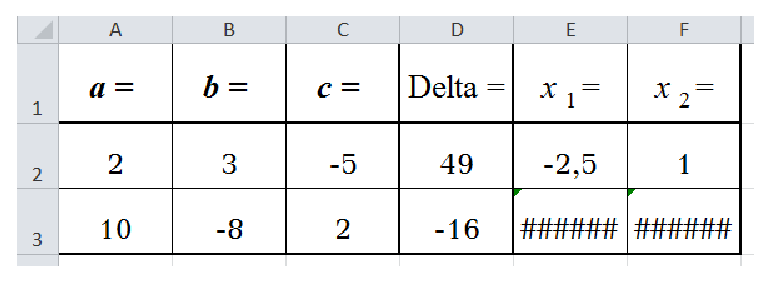
\includegraphics[scale=0.7]{Second_Degre_Excel.eps}\]
    \begin{enumerate}
        \item En détaillant les calculs, retrouver les résultats affichés dans les cellules \verb!D2!, \verb!E2! et \verb!F2!.
        \item En détaillant précisément les étapes, donner alors la factorisation du polynôme \[A(x) = 2x^2 + 3x - 5.\]
        \item Comment interpréter les symboles \verb!######! obtenus dans les cellules \verb!E3! et \verb!F3! ?
        \item On appelle $B$ le polynôme défini par les c{\oe}fficients de la ligne \verb!3!.
            \begin{enumerate}
                \item Donner l'expression du polynôme $B$ en fonction de $x$.
                \item Sans aucun calcul ni tableau de signes, en utilisant uniquement le tableur, déterminer le signe de $B$ en fonction de $x$.\par \textbf{Attention.} Une réponse non justifiée ne rapportera aucun point, même si elle est juste !
            \end{enumerate}
    \end{enumerate}
\end{exoc}\[*\]

\begin{exoc}{2 + 2 + 2 = 6 points}
    On considère la fonction polynôme $f$ telle que :
    \[\left\{\begin{array}{l}
            f(x) = ax^2 + bx + c \quad \text{pour tout } x \in \R\ ; \\
            f(0) = -1\ ;\\
            f(1) = 1,5 \quad \text{et} \\
            f(4) = 21.
    \end{array}\right.\]
    
    \begin{enumerate}
        \item Démontrer que $f(x) = x^2 + 1,5x - 1$.
        \item Résoudre l'équation $f(x) = 0$.
        \item Dresser le tableau de signes de $f$ sur $\R$ et résoudre $f(x) \geqslant 0$.
    \end{enumerate}
\end{exoc}

\vfill

\begin{center}
    \bfseries
    Tourner la page !
\end{center}

\clearpage

\begin{exoc}{1 + 1 + 1 + 2 + 3 = 8}
Dans une entreprise, les coûts de fabrication de $n$ objets sont modélisés chaque jour par  :
\[C(n) = 0,05n^2 + 0,2 n + 1\] où $n$ correspond au nombre d'objets fabriqués et le coût $C$ est exprimé en milliers d'euros.\par
La courbe représentative de $C$ est tracée ci-dessous.\par
On suppose que toute la fabrication est vendue.\medskip

\begin{center}
    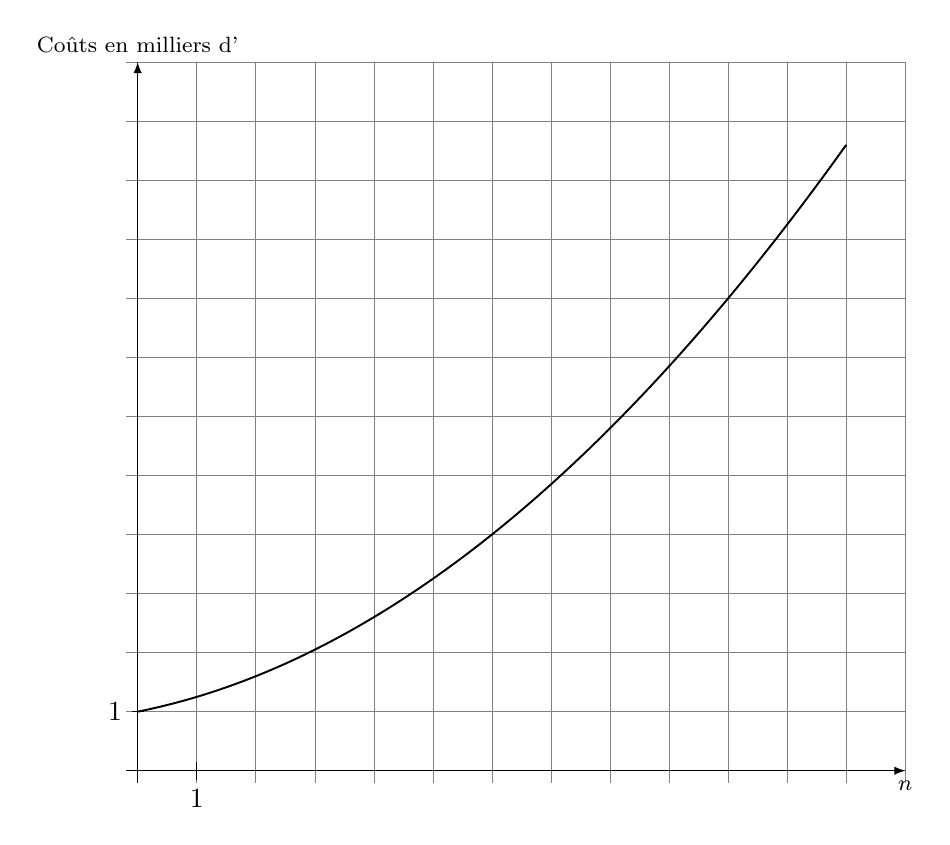
\begin{tikzpicture}[>=latex,scale=0.75]
        \draw[help lines] (-0.2,-0.2) grid (13,12);
        \draw[->] (-0.2,0) -- (13,0) node[below] {\footnotesize $n$};
        \draw[->] (0,-0.2) -- (0,12) node[above] {\footnotesize Coûts en milliers d'\EUR{}};
        \draw[line width=0.7pt] plot[domain=0:12,samples=200] (\x,{0.05*(\x)^2 + 0.2*\x + 1});
        \draw (1,0.15)--(1,-0.15) node[below] {$1$};
        \draw (0.1,1)--(-0.1,1) node[left] {$1$};
    \end{tikzpicture}
\end{center}

\begin{enumerate}
    \item À l'aide du graphique :
        \begin{enumerate}
            \item déterminer le coût de production de $10$ objets.
            \item écrire sous forme d'un intervalle le nombre d'objets à produire pour que le coût soit inférieur ou égal à \EUR{$\np{4000}$}.
        \end{enumerate}
    \item Aujourd'hui, l'entreprise a produit $9$ objets. \textbf{Calculer} le coût de production exact ?
    \item \textbf{Calculer} $C(0)$. En donner une interprétation concrète.
    \item La recette journalière est donnée par $R(n) = 0,8n$.
        \begin{enumerate}
            \item \textbf{Calculer} la recette obtenue pour $0$ objets vendus ? Est-ce rentable pour l'entreprise ? Expliquer pourquoi.
            \item \textbf{Calculer} la recette obtenue pour $10$ objets vendus ? Est-ce rentable pour l'entreprise ? Expliquer pourquoi.
        \end{enumerate}
    \item On note $B(n)$ l'expression donnant le bénéfice en fonction du nombre $n$ d'objets produits.
        \begin{enumerate}
            \item En détaillant précisément les étapes, démontrer que $B(n) = -0,05 n^2 + 0,6n - 1$.
            \item En détaillant précisément les étapes, démontrer que le bénéfice est maximal lorsque l'entreprise produit $6$ objets.
            \item Calculer alors le bénéfice pour $6$ objets produits et vendus.
        \end{enumerate}
\end{enumerate}


\end{exoc}

\end{document} 